\chapter{Introduction}
\section{Monocular Visual Odometry}
The following report describes a completely monocular visual odometry (VO) pipeline. It relies on the input of a single visual sensor to estimate a trajectory which is valid up to an unknown scale factor.

\section{Overview}
\label{params}
Before starting our VO pipeline by executing the file \emph{main.m}, the tester may choose the data set and whether or not bundle adjustment and/or trajectory alignment to the ground truth should be performed. These can be adjusted in the \emph{Configuration Section} and are summarized in Table \ref{table:params}. 

% control parameters
\begin{table}[]
\centering
\caption{Summary of control parameters}
\label{table:params}
\begin{tabular}{lll}
\hline
\multicolumn{1}{c}{\textbf{Parameters}} & \textbf{Possible values} & \textbf{Description}                                                                                                  \\ \hline
dataset\_id                             & 0, 1, 2, 3               & \begin{tabular}[c]{@{}l@{}}chooses between KITTI (0), Malaga (1), \\ parking (2) and Vespa (3) data set.\end{tabular} \\ \hline
bundle\_adjustment                      & 0, 1                     & turns on bundle adjustment                                                                                            \\ \hline
align\_to\_ground\_truth                & 0, 1                     & turns on alignment to ground truth                                                                                    \\ \hline
\end{tabular}
\end{table}
% //////

Once the pipeline is running an overview detailing the various operation parameters can be seen. A typical overview is shown in figure \ref{fig:overview}. 

% graphics of general overview
\begin{figure}[H]
  \centering
    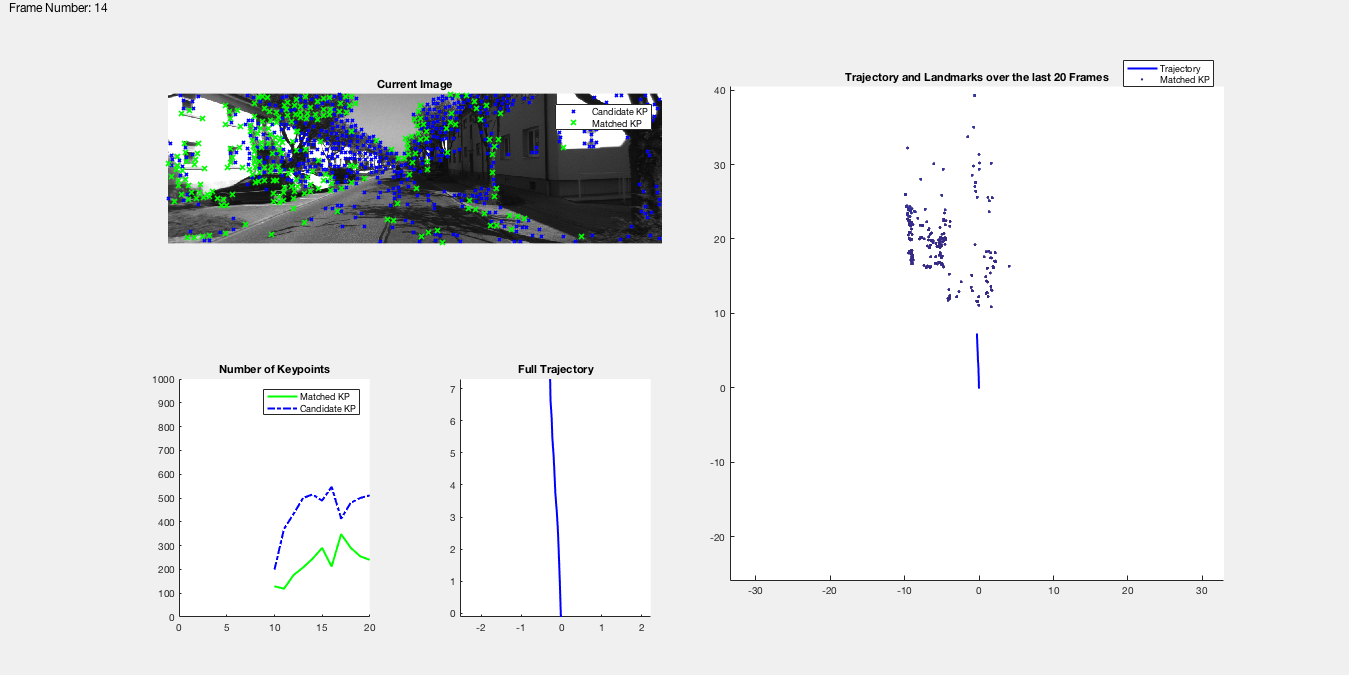
\includegraphics[width=0.5\textwidth]{figures/overview}
  \caption{Overview of the operation parameters of the VO pipeline. The current frame can be seen in the top left with the matched key points in green and candidate key points in blue. The bottom left plot shows the number of tracked candidates and matched key points over time while the bottom middle plot shows the full estimated trajectory. The right plot shows a snapshot of the trajectory as it progresses together with the matched landmarks.}
  \label{fig:overview}
\end{figure}
% //////

\section{Additional Work}
The implementation of the VO pipeline involved the tuning of several parameters which were vital to its stable performance. This was done by performing a quantitative simulation of the pipeline on the KITTI data set in order to find the combination that leads to the best trajectory estimate. For this a performance metric consisting of the average trajectory deviation from the ground truth was defined to quantify the quality of the trajectories. More on this analysis can be found in section \ref{simulation}. \par
For the purpose of testing these ideal parameters we recorded an own video which we used to validate the existing VO pipeline. This is an important test, because it guards agains over-fitting our parameters to the benchmark data sets. More information on the data set can be found in section \ref{dataset}. \par
Unfortunately scale drift is inevitable in a VO pipeline due to errors in the pose and landmark estimates. To combat this drift multiple views can be refined using bundle adjustment (BA). We integrated a form of sliding window and overlapping bundle adjustment into the existing pipeline in order to refine both structure and motion. The adjusted estimates are significantly more accurate but take longer to compute. For a more detailed discussion see section \ref{bundle adjustment}.
